%% Recipes_Detector.tex
%% Created:     Tue Apr  4 16:37:17 2017 by Koehler@I-Mac
%% Last change: 2020-09-04
%%
%% subsection for Detector Recipes
%%
%%%%%%%%%%%%%%%%%%%%%%%%%%%%%%%%%%%%%%%%%%%%%%%%%%%%%%%%%%%%%%%%%%%%%%%%%%%%%
\subsection{Detector calibration recipes}
\label{Sec:detector_calibration}

METIS will have three focal plane detector arrays:
\begin{itemize}
\item One $2\mathrm{k}\times 2\mathrm{k}$ HAWAII2RG detector used for
  LM-band imaging and slit spectroscopy.
\item One $2\mathrm{k}\times 2\mathrm{k}$ GeoSnap (Teledyne) detector
  used for N-band imaging and slit spectroscopy.
\item An array of four $2\mathrm{k}\times 2\mathrm{k}$ HAWAII2RG
  detectors used for LM-band integral-field spectroscopy.
\end{itemize}
This section lists recipes that calibrate detector characteristics
independent of a specific instrument mode. Where \FITS{_det} appears
in FITS keywords of input or product files, it is taken to mean
\FITS{_2RG}, \FITS{_GEO} or \FITS{_LMS} according to the detector
array for which data are being processed.


% \subsubsection{Detector linearity and gain determination}
% \label{sssec:metis_det_lingain}
%
% The recipe determines detector (non-)linearity and possibly detector
% gain from a set of flat-field frames taken with the broad-band lamp
% over a range of detector exposure times (DITs) and flux levels. The
% recipe structure will be similar as for \REC{detmon_ir_lg}
% \cite{detmon-manual}.
%
% The linearity curve is given by the background level as a function of
% exposure time. For each pixel the coefficients of a polynomial fit
% (order TBD) will be recorded in a coefficient cube, which can in turn
% be used to correct for non-linearity in other recipes. Pixels whose
% coefficients differ significantly from the majority of pixels will be
% marked as bad.
%
% Detector gain is typically computed pixelwise as the slope of a linear
% fit of the variance against the mean (or median) values over a set of
% frames taken over a range of DITs and illumination levels.  For
% mid-infrared detectors, in particular the Aquarius detector, this
% approach does not work due to the presence of Excess Low Frequency
% Noise (ELFN). Plotting variance against mean may be useful for
% instrument quality checks, but does not yield a meaningful value for
% detector gain. It remains to be investigated whether a different
% algorithm can be used to derive gain values.
%
% %% The sequence of increasing illumination includes an exposure with
% %% WCU window closed, this is a 'dark', capturing thermal emission
% %% within the instrument. This is subtracted from all other exposures
% %% in the sequence.
% %% This seems too much detail for the PDR doc, hence not included yet.
%
% \begin{recipedef}
%   Recipe name:         & \REC{metis_det_lingain}                                                             \\
%   Purpose:             & determine non-linearity and gain of the detectors                                   \\
%   Requirements:        & \REQ{METIS-5997}                                                                    \\
%   Type:                & Calibration                                                                         \\
%   Templates:           & \TPL{METIS_img_lm_cal_DetLin}                                                       \\
%                        & \TPL{METIS_img_nq_cal_DetLin}                                                       \\
%                        & \TPL{METIS_ifu_cal_DetLin}                                                          \\
%   Input data:          & set of \FITS{FLAT,LAMP} frames taken with increasing DIT/illumination               \\
%                        & instrument dark (\FITS{FLAT,OFF})                                                   \\
%   Algorithm:           & Subtract instrument dark                                                            \\
%                        & Compute mean and variance for each frame.                                           \\
%                        & Gain is determined as the slope of variance against mean.                           \\
%                        & Fit polynomial of value as a function of DIT and illumination level for each pixel. \\
%                        & Flag pixels with coefficients significantly different from the mean of all pixels.  \\
%   Output data:         & \PROD{GAIN_MAP_det}                                                                 \\
%                        & \PROD{LINEARITY_det}                                                                \\
%                        & \PROD{BADPIX_MAP_det}                                                               \\
%   Expected accuracies: & TBD                                                                                 \\
%   QC1 parameters:      & \QC{QC LIN GAIN MEAN}                                                               \\
%                        & \QC{QC LIN GAIN RMS}                                                                \\
%                        & \QC{QC LIN NUM BADPIX}                                                              \\
% \end{recipedef}
%
% \begin{figure}[hb]
%   \centering
%   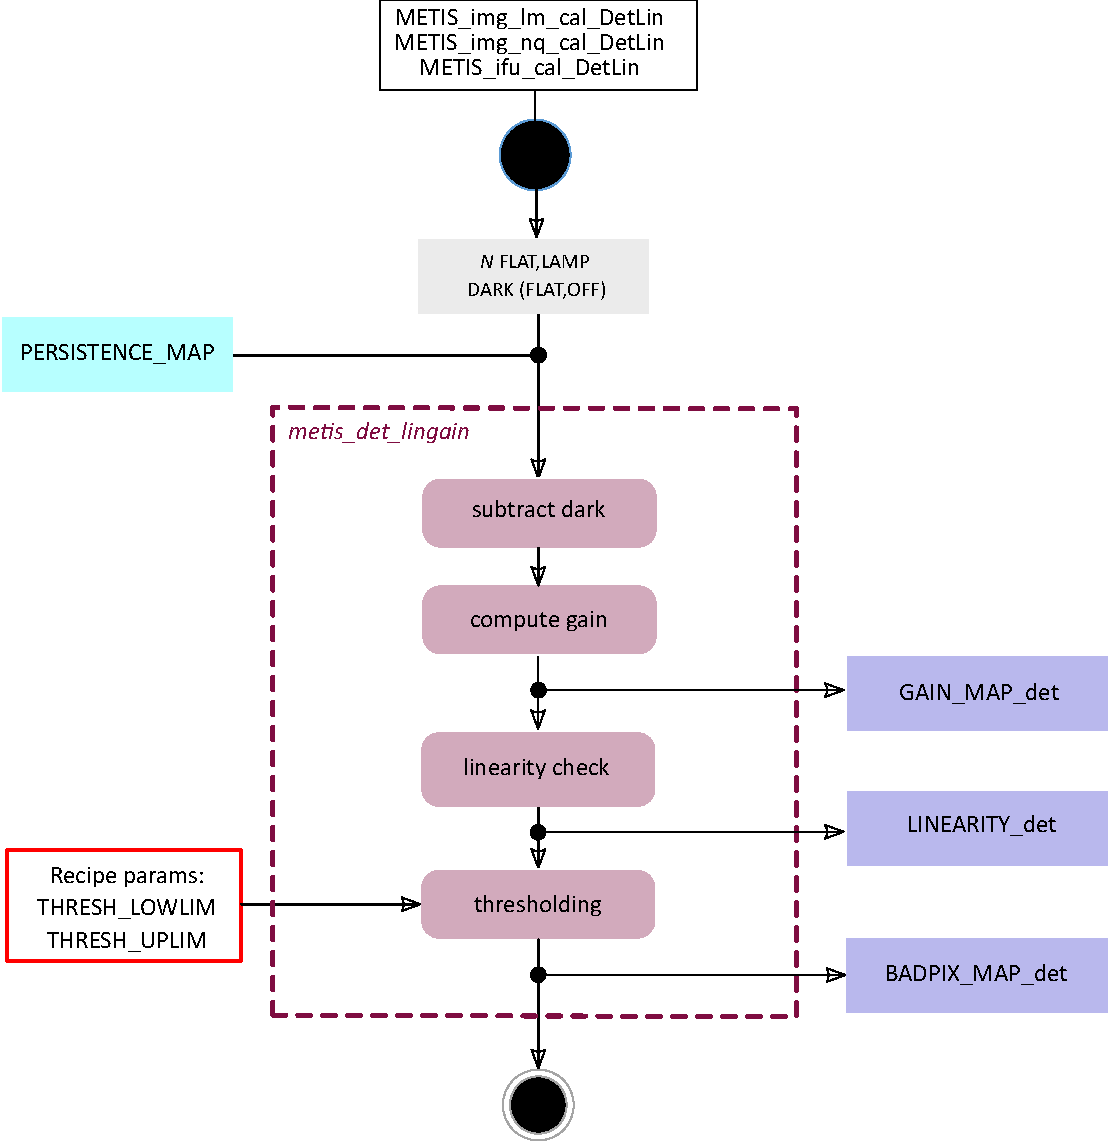
\includegraphics[width=0.65\textwidth]{metis_det_lingain}
%   \caption[Recipe: \REC{metis_det_lingain}]{\REC{metis_det_lingain} --
%     determination of linearity and gain of the detectors.}
%   \label{Fig:rec_det_lingain}
% \end{figure}
%
% %\newpage
% %\subsubsection{Excess Low Frequency Noise (ELFN)}
% %\newpage
% %\subsubsection{Masked detector area}


\newpage
\subsubsection{Master dark}
\label{sssec:metis_det_dark}

Darks are taken in daytime for all science detectors
\cite{METIS-calibration_plan}. The data will be classified by detector
(e.g.~\FITS{DET.ID} and \FITS{DET.CHIP.ID}) and exposure time
(\FITS{DET.DIT} and \FITS{DET.NDIT}). There will be ``METIS-dark''
(with the CLOSED position of the CFO-PP1 wheel) and ``Imager-dark''
(with the CLOSED position in the subsystem PP1), to be distinguished
by keyword \TBD. The former will be used for pipeline processing, the
latter for monitoring purposes.

Each set of raw dark frames is processed into a master dark. The
recipe also produces bad pixel mask by identifying cold, hot or
deviant (i.e.~hot or cold) pixels whose dark current differs
significantly (by more than $\pm 5\sigma$) from the average over the
detector.

\begin{recipedef}
  Name:                & \REC{metis_det_dark}                                                        \\
  Purpose:             & determine the dark current of the detectors                                 \\
  Requirement:         & \REQ{METIS-6063}                                                            \\
  Type:                & Calibration                                                                 \\
  Templates:           & \TPL{METIS_all_cal_dark}                                                    \\
  Input data:          & A set of DARK frames from the same detector with the same integration time. \\
  Parameters:          & Combination method (\texttt{median}, \texttt{mean},
                         \texttt{sigclip},\dots)                                                  \\
                       & Parameters for combination methods                                          \\
                       & Threshold for bad-pixel identification                                      \\
  Algorithm:           & Compute median or average of input frames to improve statistics.            \\
                       & Flag deviant pixels in master dark.                                         \\
  Output data:         & \PROD{MASTER_DARK_det}                                                      \\
                       & \PROD{BPM_COLD_det}                                                         \\
                       & \PROD{BPM_HOT_det}                                                          \\
                       & \PROD{BADPIX_MAP_det}                                                          \\
  Expected accuracies: & \TBD                                                                         \\
  QC1 parameters:      & \QC{QC DARK MEAN}                                                              \\
                       & \QC{QC DARK MEDIAN}                                                            \\
                       & \QC{QC DARK RMS}                                                               \\
                       & \QC{QC DARK NBADPIX}                                                             \\
                       & \QC{QC DARK NCOLDPIX}                                                               \\
                       & \QC{QC DARK NHOTPIX}                                                                \\
                       & (more \TBD)                                                                  \\
\end{recipedef}

\begin{figure}[hb]
  \centering
  \includegraphics[width=0.5\textwidth]{metis_det_dark.pdf}
  \caption[Recipe: \REC{metis_det_dark}]{\REC{metis_det_dark} -- creation of master
    dark and bad pixel maps}
  \label{Fig:rec_det_dark}
\end{figure}

\clearpage
%%%%%%%%%%%%%%%%%%%%%%%%%%%%%%%%%%%%%%%%%%%%%%%%%%%%%%%

%%% Local Variables:
%%% TeX-master: "METIS_DRLD"
%%% End:
